\documentclass{bioinfo}
\copyrightyear{2015} \pubyear{2015}


\usepackage{natbib}
\usepackage{algorithm}
\usepackage{algorithmic}
\usepackage{amsmath}
\usepackage{amssymb}
\usepackage{bbm}
\usepackage{xspace}
\usepackage{subfiles}

\newcommand{\parent}{\text{parent}}
\newcommand{\pd}[2]{\frac{\partial #1}{\partial #2}}
\newcommand{\nut}{\tilde{\nu}}
\newcommand{\Mt}{\tilde{M}}
\newcommand{\Poisson}{\mathrm{Poisson} }
\newcommand{\Beta}{\mathrm{Beta} }
\newcommand{\ancestors}{\mathrm{An} }
\newcommand{\descendants}{\mathrm{De} }
\newcommand{\bancestors}{\overline{\ancestors}}
\newcommand{\Uniform}{\mathrm{Uniform} }

\newcommand{\Categorical}{\mathrm{Categorical} }
\newcommand{\Multinomial}{\mathrm{Multinomial}}
\newcommand{\Binomial}{\mathrm{Binomial}}
\newcommand{\NegativeBinomial}{\mathrm{NegativeBinomial}}
\newcommand{\Bernoulli}{\mathrm{Bernoulli} }
\newcommand{\Dirichlet}{\mathrm{Dirichlet} }
\newcommand{\InvWishart}{\mathrm{InvWishart} }
\newcommand{\Wishart}{\mathrm{Wishart} }
\newcommand{\Geometric}{\mathrm{Geometric}}

\newcommand{\bx}{{\bf x}}
\newcommand{\by}{{\bf y}}
\newcommand{\hy}{\hat{y}}
\newcommand{\hL}{\hat{\Lambda}}
\newcommand{\nth}{\textsuperscript{th}\xspace}

\newcommand{\tnu}{\tilde{\nu}}
\newcommand{\td}{\tilde{d}}
\newcommand{\tv}{\tilde{t}}
\newcommand{\ind}{\mathbbm{1}}
\newcommand{\B}{\mathrm{B}}

\access{Advance Access Publication Date: Day Month Year}
\appnotes{Manuscript Category}

\begin{document}
\firstpage{1}

\subtitle{Subject Section??}

\title[Tumor Subclonal Reconstruction with Aldous' Beta-Splitting]{Tumor Subclonal Reconstruction with Aldous' Beta-Splitting}
\author[Sample \textit{et~al}.]{Levi Boyles\,$^{\text{\sfb 1,}*}$, Amit Deshwar\,$^{\text{\sfb 2}}$, Quaid Morris\,$^{\text{\sfb 2}}$, Max Welling\,$^{\text{\sfb 3}}$, Yee Whye Teh\,$^{\text{\sfb 1}}$  }
\address{$^{\text{\sf 1}}$Department of Statistics, University of Oxford, Oxford, OX1 3TG, United Kingdom and \\
$^{\text{\sf 2}}$Department, Institution, City, Post Code,
Country and \\
$^{\text{\sf 3}}$Informatics Institute, University of Amsterdam, Amsterdam, 1098 XH, The Netherlands.}

\corresp{$^\ast$To whom correspondence should be addressed.}

\history{Received on XXXXX; revised on XXXXX; accepted on XXXXX}

\editor{Associate Editor: XXXXXXX}

\abstract{\textbf{Motivation:} 
We develop beta-splitting trees, first introduced by Aldous, as Bayesian models for the problem of tumor subclonal reconstruction.  Due to the complex discrete-continuous nature of the model, posterior simulation is quite involved and we develop a Markov chain Monte Carlo methodology based on Hamiltonian Monte Carlo, reversible jump, and the Wang-Landau algorithm.
\\
\textbf{Results:} CPABS is shown to provide better reconstructions than other tools in a variety of scenarios.\\
\textbf{Availability:} Software is available in the CPABS package for the Julia technical computing language: https://github.com/leviboyles/cpabs\\
\textbf{Contact:} \href{boyles@stats.ox.ac.uk}{boyles@stats.ox.ac.uk}\\
\textbf{Supplementary information:} Supplementary data are available at \textit{Bioinformatics}
online.}

\maketitle

\section{Introduction}

One of the leading models for tumor evolution is the \emph{subclonal} model, in which a tumor is a heterogeneous population comprised of multiple subpopulations (or subclones) with different selective advantages \cite{Pritchard2000, Shah2012, Jiao2014}.  These subpopulations are characterized by driver mutations, which are in turn associated with cancer development  \cite{Hanahan2000, Hanahan2011}, and related to each other via a phylogeny which describes the evolutionary history of the tumor.  The task of subclonal reconstruction is to establish the subclonal composition of a tumor from high throughput sequencing data, with the aim of providing insights into potential treatment options \cite{Aparicio2013, Bedard2013}.

There are a number of existing methods for subclonal reconstruction.  (TODO: non Bayesian approaches?) \cite{Shah2012} models subclones with a ``flat clustering'' model -- there is no explicit parent/child relationship between subclones defined by the model.  \cite{Jiao2014} provides a model allowing for hierarchical interpretations of the subclonal composition, utilizing Tree Structured Stick Breaking (TSSB) \cite{adams2010tssb}, a Bayesian prior on trees. 

In this work, we explore a model utilizing Beta-Splitting trees \cite{Aldous1995} as a prior for the subclonal hierarchy.  There are many choices for a prior distribution on latent tree structures for Bayesian modelling.  Often it is desirable that these prior distributions possess particular properties that make them well suited to the problem at hand.  For example, in hierarchical clustering it is often useful to choose a prior that prefers balanced trees over imbalanced ones in order to encourage sharing of statistical strength across clusters.  Beta-splitting trees enjoy a number of useful properties, including projectivity, flexibility in modelling both balanced and imbalanced trees, and are related to a number of existing tree models, including the uniform tree distribution and Kingman's coalescent.  We introduce consistent time variables for these trees that can capture the inverse relationship between subpopulation size and mutation number.  Additionally, there are some computational benefits over other choices of prior such as Kingman's coalescent.

In Section \ref{sec:likelihood}, we describe our model for the evolutionary history of a tumor, given a tree describing the shape of the phylogeny.  Section \ref{sec:beta_splitting} reviews our prior on phylogenies, namely Aldous' beta-splitting.  Section \ref{sec:related} we review related prior distributions.  In Section \ref{sec:inference} we describe the inference methodology used, and in Section \ref{sec:experiments} we compare our model against a state-of-the-art model for subclonal reconstruction.  Finally, we conclude in Section \ref{sec:conclusions}. 

\begin{methods}

\section{Subclonal Reconstruction}
\label{sec:likelihood}
Consider the following generative description of tumor evolution (see also Figure \ref{fig:tumor_evolution}):
\begin{enumerate}
\item Given a large population of cells, any individual cell lineage acquires ``driver mutations'' -- single-site mutations (SSMs) associated with cancer -- with mutation rate $\lambda_d$, and ``passenger mutations'' with mutation rate $\lambda_p$. Passenger mutations are those introduced by the enhanced growth of the tumor but are selectively neutral.
\item When a cell acquires a driver mutation, the resulting descendent subpopulation becomes a significant proportion of the overall population.  All cells in the descendant subpopulation have the driver mutation as well as all passenger mutations associated with that driver.
\item We observe only mutations that are present in entire subpopulations with a significant proportion of the overall population. 
\end{enumerate}
The data are gathered from a deep read sequencing of a tumor biopsy, with multiple coverage per site ({\bf better term/phrasing for this?}) .  We assume that the only mutations we observe with high enough frequency to be distinguished from noise are driver mutations and passenger mutations who precede a driver mutation on a cell lineage.  Additionally, we make an infinite sites assumption: no mutation event will introduce an SSM that is already present elsewhere in the tumor, nor will it remove any SSMs.  

For a particular tumor, we have a finite set of $M$ mutations.  We may have biopsied the tumor multiple times giving a number of samples $S$.  We observe the number of reads $d_{m,s}$ covering the location of mutation $m$ in sample $s$.  Out of these, $b_{m,s}$ are observed to have the mutation, and thus $a_{m,s} = d_{m,s}-b_{m,s}$ do not.


\begin{figure}
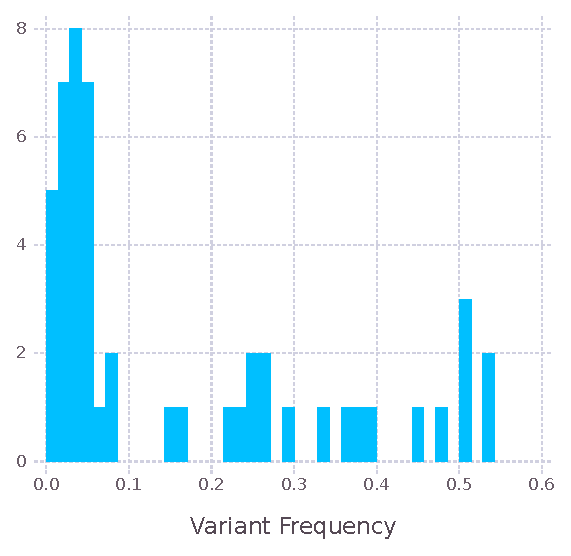
\includegraphics[width=0.9\columnwidth]{../figures/simulated_data.eps}
\caption{Variant mutation frequency histogram for an example simulated dataset.  The x-axis corresponds to the population frequency for each mutation, specifically we plot $b_m/d_m$ for each mutation.  There are five ground truth clones in this dataset, three of which share the low-frequency end of the histogram.}
\label{fig:data}
\end{figure} 


The aim of the reconstruction task is to infer the set of subpopulations that comprise the tumor and the assignment of mutations to the subpopulations from which they originated.  In many models for subclonal reconstruction, the latent subpopulations are related to the data by modelling the \emph{cellular prevalence} of each subpopulation, that is, the proportion of cells that are descendants of that subpopulation.  Cellular prevalence is clearly related to the variant counts $b_{m,s}$ -- we would expect to see larger variant allele frequencies (VAFs) $b_{m,s}/d_{m,s}$ for mutations associated with larger subpopulations.  A key distinction between existing subclonal reconstruction tools is in the way in which the cellular prevalences, hereon denoted $\phi$, are modelled.  PyClone \cite{Roth2014} models the cellular prevalences with a Dirichlet process, assuming a flat clustering model for the mutations.  PhyloSub \cite{Jiao2014} introduces a latent hierarchy that models the nested structure of the subpopulations, requiring that the cellular prevalence of a parent subpopulation is greater than that of the sum of cellular prevalences of its children.  In these models, the reference read counts, are modelled given the cellular prevalences.  If $\phi_{k,s}$ is the cellular prevalence for subpopulation $k$ in sample $s$, $z_m$ is the subpopulation to which mutation $m$ belongs, and $\eta_m^r$ and $\eta_m^v$ are the probabilities of observing a reference read from the reference and variant populations, respectively\footnote{Typically, $\eta^r \approx 1.0$ and $\eta^v \approx 0.5$, accounting for the possibility of reading the non mutated chromatid in a variant type cell.}, then the reference count is modelled by: 

\begin{equation}
\label{eq:refcount}
a_{m,s} \sim \Binomial(d_{m,s}, (1-\phi_{z_m,s})\eta_m^r + \phi_{z_m,s}\eta_m^v).
\end{equation}

\begin{figure}
\centering
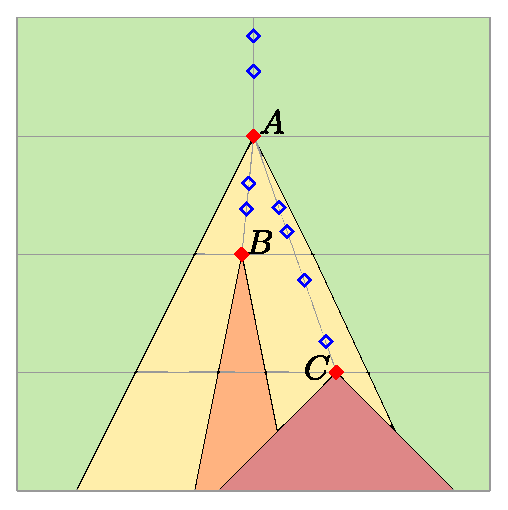
\includegraphics[width=0.9\columnwidth]{../figures/tumor_subclonal_growth_A.eps}
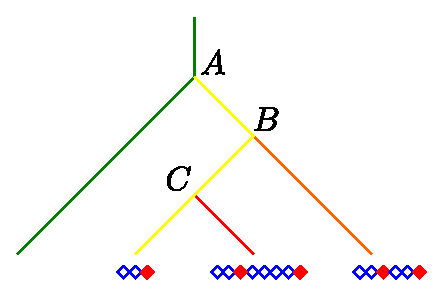
\includegraphics[width=0.9\columnwidth]{../figures/tumor_subclonal_growth_B.eps}
\caption{Assumed process for tumor evolution (best viewed in color).  The process begins with a single lineage within a reference population (green area) which acquires passenger mutations (blue diamonds) over time.  Eventually, this lineage acquires a driver mutation (red-filled diamonds) that spawns a new subpopulation $A$ that begins to compete with the reference population.  This occurs 2 more times, spawning from within the $A$ subpopulation to create two additional subpopulations $B$ and $C$.  This particular outcome corresponds to the binary tree shown below, if right subtrees correspond to newly spawned subpopulations and the left subtrees correspond to old subpopulations.  Each colored line corresponds to the path from each population at the leaves to its point of divergence from its parent population.  The length of the path from the divergence point to the earliest ancestor that can be reached from a path of a single color is the time available for the population to acquire passenger mutations.  The mutations associated with a population are depicted at that population's leaf.}
\label{fig:tumor_evolution}
\end{figure}

\subsection{Mutation Model}

We extend the latent representation used to model tumor evolution to include time variables in addition to a discrete hierarchy, where there is time $t_i$ associated with each node $i$ in the hierarchy.  These times are used to model the number of passenger mutations that occur between driver events.  These time variables are not to be interpreted as physical time; the physical times and mutation rates of each subpopulation are not identifiable given the mutation read counts.  Instead, time between two nodes can be interpreted as the product of the physical time between the driver events and the mutation rate of the subpopulation spawned from the parent driver event.  In other words, the times variables $t_i$ can be interpreted as time rescaled to a globally constant mutation rate.

Let $\pi$ denote a binary tree, and let $\psi = (\pi, \{t_i\})$ denote the collection of the tree along with the time variables.  Beta splitting defines a prior on $\psi$, and  Section \ref{sec:beta_splitting} defines this prior; we first consider the likelihood model for the data given a draw from this prior.  For a binary tree $\pi$, we will index the set of nodes by strings in $\{l,r\}^*$, with the root being the empty string $\epsilon$, and for each $i$ in $\{l,r\}^*$ its two children being $il$ and $ir$.  

%We introduce a set of rate variables that govern the distribution of the number of mutations that occur at each node.
%
%Let $\tau(i)$ be the most recent ancestor of node $i$ from which the subtree containing $i$ is the right subtree, that is, $\tau(i)$ is the parent subpopulation of subpopulation $i$.  Thus $v_i = t_{\tau(i)} - t_i$ is the time after which the subclone associated node $i$ spawned from its parent subpopulation $\tau(i)$.  
%
%Let $\lambda_i$ be the passenger mutation rate associated with node $i$.  This is generated according to a Gamma with scale $v_i$.
%
%\begin{equation} \lambda_i \sim \Gamma(k, v_i) \end{equation}
%
%Then, the vector of passenger mutation counts $u_i$ is drawn according to a Multinomial:
%
%\begin{equation} u \sim \Multinomial(\frac{\lambda}{\sum_i \lambda_i}) \end{equation}

Note that the subpopulation hierarchy is not necessarily binary, but our prior is over binary trees $\pi$.  Thus we make a distinction between the binary tree $\pi$ and the subpopulation hierarchy $H$ (a multifurcating tree,) and relate the two in the following way.  A node $i$ in $\pi$ has the subpopulation $h_i \in H$ associated with it.  The right and left subtrees of a node $i$ are treated differently, the right subtree corresponds to the new subpopulation $h_{i}$ which has acquired a cluster of SSMs and the left subtree corresponds the old subpopulation $h_{\parent(i)}$ without any new SSMs.  This is the natural result of applying a binary tree prior to this problem, see Figure \ref{fig:tumor_evolution}.  Thus, the parent node $\parent(i)$ does not necessarily correspond to the parent population of the population associated with node $i$, that is it is \emph{not} necessary that $h_{\parent(i)} = \parent(h_i)$. 

Let $\tau(i)$ be the most recent ancestor of node $i$ from which the subtree containing $i$ is the right subtree.  Thus, $\tau(i)$ is the node associated with the parent population of subpopulation $i$: $h_{\tau(i)} = \parent(h_i)$.  Then $v_i = t_{\tau(i)} - t_i$ is the time after which the subclone associated with node $i$ spawned from its parent subpopulation at $\tau(i)$.  We assume passenger mutations occur according to a Poisson process, so that under the generative process we have that the number of passenger mutations associated with population $i$ is $u_i \sim \Poisson(\lambda_p v_i)$. However, the total number of passenger mutations is known for a given tree, so the vector of passenger mutation counts $u_i$ is distributed according to a Multinomial:

\begin{equation} u \sim \Multinomial\left(M, \frac{v}{\sum_i v_i}\right). \end{equation}

Let $z_m=i$ if mutation $m$ belongs to population $h_i$.  There are two ways a mutation may have been assigned to a population, either as a driver mutation, or a passenger mutation.  Let $K=N-1$ be the number of driver mutations, then we have

\begin{equation}
p(z_m=i|\psi) = \frac{K}{M}\frac{1}{K} + \frac{M-K}{M} \frac{v_i}{\sum_j v_j} = \frac{1}{M} + \frac{M-K}{M} \frac{v_i}{\sum_j v_j}.
\end{equation}
 
\subsection{Modelling Subpopulation Sizes and Read Counts}
In practice, only a subset of the tumor is biopsied, and this may be performed multiple times giving multiple ``samples'' of the tumor.  Following \cite{Pritchard2000}, we model each sample as an admixture of the subclonal populations, with differing mixing proportions for each sample.  This reflects the heterogeneity of the composition of each sample.

The SSM population frequency $\phi_{i,s}$ for population $i$ and sample $s$ are constructed as 
\begin{equation}
\phi_{i,s} = \upsilon_{ir,s} \prod_{j \in \bancestors(i) } \upsilon_{j,s} \;\;\;\;\;\;\;\;\;\;\;\;\; \upsilon_{j,s} \sim \Beta(\alpha\nu_j + 1, \alpha(1-\nu_j) + 1) \label{eq:obs}.
\end{equation}

where $\bancestors(i) = \ancestors(i) \cup \{i\}$.  $\alpha$ is a hyperparameter of the model, and $\upsilon_{jl,s} = 1-\upsilon_{jr,s}$.  Larger values of $\alpha$ will shrink the variance of $\upsilon_{j,s}$, so that the proportions for each sample more closely match the beta-splitting proportions.  Note that $\upsilon_{j,s}$ is uniformly distributed when $\alpha=0$.  Thus, the $\phi$ variables are more strongly tied across samples than if they were treated as independent variables when $\alpha > 0$.  This will still enforce the SSM population constraints, that is, $\phi_{il,s} \leq \phi_{i,s}$ and $\phi_{ir,s} \leq \phi_{i,s}$.   

Finally, given $\phi$ and a number of reads $d_{m,s}$, we draw the number of reference reads $a_{m,s}$ as in \eqref{eq:refcount}.

\begin{figure}
\centering
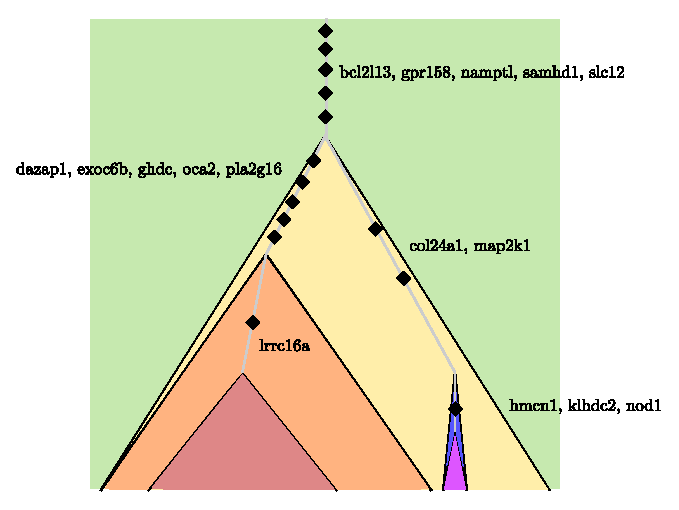
\includegraphics[width=0.9\columnwidth]{../figures/CLL_growth_cartoon.eps}
\caption{Representative sample from the posterior for the CLL077 dataset.  The width of each subpopulation at the base of the figure reflects the cellular prevalence of that subpopulation.  Also shown are the unique mutations associated with each subclone.  Time variables are not accurately depicted in this figure.}
\label{fig:CLL_result}
\end{figure} 


\section{Beta-Splitting Trees}
\label{sec:beta_splitting}
Beta-splitting defines an infinite tree-structure in a top-down fashion.  Let $f(x)$ be a symmetric density on the unit interval.  Begin by placing $N$ points, or individuals, uniformly at random on the unit interval; let $y_i$ denote the location of point $i$.  Then repeat until all points are isolated:
\begin{enumerate}
\item Draw $x \sim f$.
\item Individuals with $y_i < x$ are designated to the left branch, all others designated to the right. 
%\item Draw $l_i \sim \Bernoulli(x)$ for each point $i$
%\item Those $i$ with $l_i=1$ are designated to the left branch, all others designated to the right
\item Recurse on each subinterval (after rescaling each to a unit interval), until all points are assigned their own branches as leaves. 
\end{enumerate}
See Figure \ref{fig:aldous_betasplit} for an illustration.  This process defines an infinite tree if we let $N\rightarrow \infty$.  \cite{Aldous1995} specializes $f$ to a one-parameter Beta distribution, so that $x \sim \Beta(\beta+1,\beta+1)$. Picking $\beta$ and marginalizing out $x$ for $-2 \leq \beta < \infty$ (the discrete distribution on trees obtained by integrating out $x$ is still sensible for $-2 \leq \beta \leq -1$) gives rise to many familiar priors, for example $\beta=0$ corresponds to Kingman's Coalescent prior, and $\beta=-\frac{3}{2}$ corresponds to the uniform distribution on trees.

%Typically, $x$ is integrated out and the resulting discrete distribution over tree structures remains, with an additional time variable for each internal node representing the time at which a set of leaves' lineages split.  However, we will instead represent the splitting proportions $x$.  Thus the $N$ points are conditionally independent given the splits, allowing for more efficient inference.  Additionally, representing the splitting proportions gives a convenient way to define the times of the internal nodes of the tree.



%We will identify a node of a tree with a string indicating the path that leads to the node from the root.  Thus the root is identified with the empty string (denoted $\epsilon$), and its left and right children is identified with $l$ and $r$, respectively.  Further descendants are identified by appending $l$ or $r$ to its parent's index, as appropriate.  In the following, we will use $i$ or $j$ to denote the string associated with an arbitrary node.
%
%We are interested in representing beta-splitting trees restricted to a finite set of $N$ points, that is, trees with $N$ leaves.  In the following, the indices $i$ refer to nodes in such a tree.
%Let $\nu_i \sim \Beta(\beta+1,\beta+1)$ be the splitting proportion associated with node $i$, and $\mu_i$ be the total proportion of mass associated with the subtree rooted at node $i$, as drawn from the beta-splitting process.   
%
%In the beta-splitting process, a finite set of $N$ points may not be separated by the drawn splitting point, thus causing a split in the infinite tree that is not represented in the tree restricted to the $N$ points.  Thus, with finite $N$, $\mu_i$ is not simply $\nu_i\prod_{j \in \ancestors(i)} \nu_j$, where $\ancestors(i)$ is the ancestor set of $i$ -- we must account for these splits that may have occurred without separating our finite set of points.  Consider node $i$ with children $il$ and $ir$, where $N_i$ points split into two sets of sizes $N_{il}$ and $N_{ir}$.  Let $\nut_i$ be the total split proportion accumulated by repeated beta-splitting of the $N_i$ points until a split actually occurs.  We derive the distribution of $\nut_i$ next, see Figure \ref{fig:aldous_betasplit} for a visualization of the resulting representation. 
%
%We restrict our attention to the Coalescent model, $\beta=0$, so that $x \sim \Uniform(0,1)$.  The marginal probability of a set of $N_i$ points failing to split apart is 

In the generative process of the beta-splitting tree, it is possible that the split point $x$ may be trivial, that is, that the individual points all lie to the left of $x$, or all to the right of $x$.  In such a situation the structure of the tree, as defined by the hierarchical separation of the individuals into leaves of the tree, does not change, but the length of the interval containing the individuals does.  Let $N_i$ be the number of individuals at node $i$, $D_i$ be the number of trivial splits prior to node $i$, $\tilde{\nu}_i$ be the proportion of the original interval still containing the individual points before the non-trivial split, and $\mu_i$ be the resulting length of the interval just before the (non-trivially) split, (see Figure \ref{fig:aldous_betasplit} (right).)  Finally, let $\nu_{il}$ and $\nu_{ir}$, with $\nu_{il}+\nu_{ir}=1$, be the proportions on the left and right children of $i$ respectively.

In the case where $f$ is a uniform distribution on $[0,1]$, corresponding to Kingman's coalescent, it turns out to be possible to marginalize out both the $N$ individual locations $\{y_k\}$ and the number of trivial splits $\{D_i\}$ before each node of the tree, and derive an explicit distribution for $\tilde{\nu}_i$.  First, note that the marginal probability of failing to split a set of $N_i$ points is:

\begin{equation}
2 \int x^{N_i} (1-x)^0 f(x) dx = \frac{2}{N_i+1}.
\end{equation} 
Let $\xi_{N_i} = 1-\frac{2}{N_i+1}$. Then $D_i \sim \Geometric(\xi_{N_i})$ gives the number of failures until the $N_i$ points are split.  The distribution of $\nut_i$ is thus the product of $D_i$ uniform draws.  If we take $U_k \sim \Uniform(0,1)$, and $U^{(d)} = \prod_{k=1}^d U_k $, then $-\ln U^{(d)}$ is the sum of $d$ Exponential draws, thus $- \ln U^{(d)} \sim \Gamma(d,1)$, and so
\begin{align}
p( -\ln \nut_i = y) 
%&= \sum_{d=1}^\infty p(D_i=d) p( -\ln U^{(d)} = y) + p(D_i=0) \delta_0(y)\\
&= \sum_{d=1}^\infty (1-\xi_{N_i})^d \xi_{N_i} \frac{1}{(d-1)!} y^{d-1} e^{-y} + \xi_{N_i} \delta_0(y)\\
%&= (1-\xi_{N_i}) \xi_{N_i} e^{-y} \sum_{k=0}^\infty \frac{\left((1-\xi_{N_i})y\right)^k}{k!} + \xi_{N_i}\delta_0(y)\\
&= \xi_{N_i}\delta_0(y) + (1-\xi_{N_i}) \xi_{N_i} e^{-\xi_{N_i} y} 
\end{align}
which gives
\begin{equation}
\nut_i \sim \xi_{N_i}\delta_1(\nut_i) + (1-\xi_{N_i}) \Beta(\xi_{N_i},1) \label{eq:nut} 
\end{equation}
that is, $\nut_i$ is a mixture between a point mass at 1 and a $\Beta(\xi_{N_i},1)$.  This result agrees with intuition: if $N_i$ is large, then $\xi_{N_i}$ is close to 1, and $\nut_i$ is close to 1.  $\nu_i$ is simply $\Uniform(0, 1)$ and $\nu_{ir} = 1 - \nu_{il}$.  If $N_i$ points are split into groups of sizes $N_{il}$ and $N_{ir}$, then 
\begin{equation}
p(\nu_{il},N_{il}, N_{ir}) = \frac{2}{(N_{il} + N_{ir})(N_{il} + N_{ir} -1)} \nu_{il}^{N_{il}-1} (1-\nu_{il})^{N_{ir}-1}.\label{eq:nu_N}
\end{equation}
This form arises from the fact that we are conditioning on a split occurring, that is, $N_{il}>0 $ and $N_{ir}>0$.  Finally, we can write $\mu_i$: 
\begin{equation}
\mu_i = \nu_i \nut_i \prod_{j \in \ancestors(i)} \nu_j\nut_j. \label{eq:mu_i}
\end{equation}

In summary, we have a finite tree with $N$ leaves and each internal node having two children.  At each internal node $i$ we have $\mu_i$, the interval length before it splits, given by \eqref{eq:mu_i}, where $\nut_i$ is given by \eqref{eq:nut} and the joint distribution of the proportion of the interval and numbers of leaves of the two children of $i$ are given by \eqref{eq:nu_N}.

\begin{figure*}
\centering
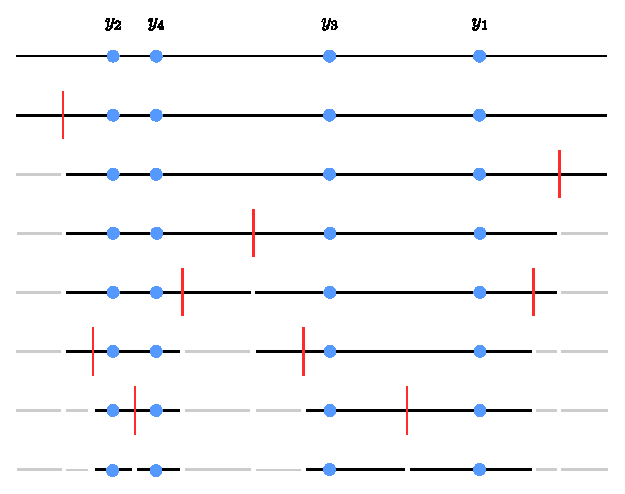
\includegraphics[width=0.9\columnwidth]{../figures/aldous_betasplit_full.eps}
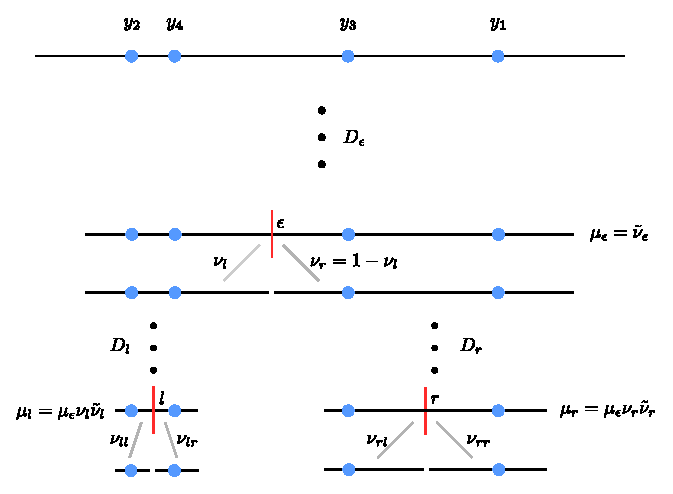
\includegraphics[width=0.974\columnwidth]{../figures/aldous_betasplit_marginalB.eps}
\caption{Aldous' Beta-splitting.  \textbf{(left)} Five points are dropped onto the unit interval, which is then recursively split according to beta-splitting.  Note that splits may occur that do not separate any data. \textbf{(right)} By marginalizing out the splits that do not separate data, we get a simplified representation for the Beta-Splitting tree using fewer explicit splitting locations.  In the figure, beta-splitting failed to separate the four points $D_\epsilon$ times, resulting in an interval of length $\nut_\epsilon$.  This interval is then split into two subintervals with proportions $\nu_l$ and $\nu_r$, and the process recurses on each subinterval.  Note that we need not explicitly represent the locations $y$ to sample from this process, as we need only determine to which subinterval each point belongs at each split event.}
\label{fig:aldous_betasplit}
\end{figure*}

%\subsection{Introducing Time Variables}
\label{sec:time}
Variables that denote the time from leaf to internal node are often employed in hierarchical clustering models.  Typically, the parameters that generate the observations reside at the internal nodes of the tree, with shorter branch lengths corresponding to stronger correlations between parameters.  If the time variables have the property that internal nodes that have few descendants are strongly encouraged to have smaller times\footnote{We take the convention that time runs from leaves to root} and thus are ``closer'' to the leaves, then the clustering model is less likely to be overly flexible and in danger of overfitting.  Kingman's Coalescent and the Dirichlet Diffusion Tree \cite{neal2003dft} both employ time variables with this property.

The choice of time variables is a delicate one, as any choice should leave the overall distribution consistent (in the Kolmogorov sense).  One way to ensure that the times retain a consistent prior distribution is to show that the time to the most recent common ancestor (MRCA) for a pair of nodes is the same in the infinite tree as it is in a finite projection.  For internal node $i$, we may define the time $t_i$ as
\begin{equation}
t_i = g(\mu_i) \label{eq:t_p}
\end{equation}
where $g$ is a monotonically increasing function with $g(0)=0$.  Thus using $\mu_i$ to define a time variable gives a consistent prior over times.  As $0 \leq \mu_i \leq 1$, choosing a strictly convex $g$ with $g(1)=1$ will correspond to nodes that are closer to the leaves, and thus to a less flexible prior. 

This choice of time variable has two main advantages over the times used for the Coalescent model.  First, the time for a node $i$ is dependent only on the number of individuals delegated to each of its children.  Coalescent times, on the other hand, are determined by starting with $N$ individuals and recursively joining pairs of with exponential waiting times -- the time for node $i$ is directly dependent on the times of many other nodes throughout the tree.  Thus, MCMC inference under Beta-Splitting can be performed in a more computationally efficient manner.  Second, this construction allows for more choice in the specification of how the times are distributed for nodes that are deeper in the hierarchy, for example the choice of $g$ can be modified to push internal nodes leaf-wards or root-wards.  Thus we obtain a prior with the same distribution on tree structures as that in Kingman's Coalescent, but with a more flexible choice as to the distribution on times.

\subsection{Number of Clones}
The above model is defined for a fixed number of clones (equivalently, for a tree with a fixed number of leaves.)  Unlike the TSSB, any two points will eventually be split by beta-splitting.  In our model, a point in the beta-splitting process corresponds to an entire population.  Thus, in order allow for a variable number of clones, we specify a prior on the $K$, namely:
\begin{equation}
K \sim \NegativeBinomial(c,\theta). 
\end{equation}
We choose $c=2$ and $\theta=0.4$ so that $K$ has a large variance. 

\section{Related Work}
\label{sec:related}

There are many choices for prior distributions over trees which have differing properties.  Perhaps the simplest prior is the uniform tree distribution, where each tree with $N$ leaves is given equal probability.  This distribution has the property in that the typical draw from the uniform prior is imbalanced \cite{Aldous1995}.  Another is the distribution on trees induced by Kingman's Coalescent \cite{Kingman82g}, in which, given $N$ individuals, pairs are \emph{coalesced} uniformly at random until a full tree is formed.  A typical draw from this distribution is balanced.  Another interesting prior is the Dirichlet Diffusion Tree (DDT) \cite{neal2003dft}, which defines a joint distribution on tree structures and time variables which cannot be factored into analytically tractable factors.  The distribution on the DDT's time variables is specified by a ``divergence function'' which also influences the balance of the tree. 

The Tree-Structured Stick Breaking (TSSB) \cite{adams2010tssb} prior allows data to sit at internal nodes of the tree, thus the size of the tree (its number of nodes) is inferred in addition to the structure.  The TSSB has been used in our problem of interest: tumor subclonal reconstruction \cite{Jiao2014}.  However, the TSSB has the tendency to prefer shallow hierarchies with high branching factors \cite{steinhardt2012martingale}, a property which is not necessarily ideal for subclonal reconstruction. 



\section{Inference}
\label{sec:inference}
\subsection{Sampling $\nu, \nut, \upsilon$, and $z$} 
We give brief descriptions of the inference methods used, for more detail on the updates for $\nu, \nut, \upsilon$, and $z$, see the supplementary appendix.

The $\nu$ variables are continuous variables with nondegenerate densities, and so we update each one in turn with slice sampling \cite{Neal2003a}.  The $\nut$ variables are continuous with an atom at 1 due to the form of the \eqref{eq:nut}.  We update each in turn, augmenting the atom with an auxiliary variable giving a nondegenerate density from which we slice sample, projecting to the atom as appropriate (this is a similar approach to that taken in some spike and slab models.)  We sample $\upsilon$ according to Hamiltonian Monte Carlo \cite{Duane1987}, as these variables are strongly tied and it is important to update them jointly.  Finally, we update $z$ according to Gibbs sampling.
\subsection{Sampling the tree structure $\psi$}
We employ a prune/graft sampling algorithm where we randomly choose a node to prune from the tree, and then sample a new location for the pruned subtree.  We hold the $\nu$ variables fixed, so grafting will change the times associated with the nodes underneath the graft point.

Sampling $\psi$ can be done in a more computationally efficient manner than in the Coalescent.  After pruning a subtree with a number of leaves $n < N$, to evaluate the posterior probability of a potential grafting location we need to evaluate the likelihood and prior for the subtree rooted at the grafting location.  For a likelihood that depends directly on the time variables (such as a Brownian motion likelihood), as the $\nu$ variables are fixed and the times are defined as products of $\nu$ variables over a node's ancestors, the posterior probabilities for all graft locations can be computed in $O(Nn)$ time using dynamic programming.  The likelihood defined by \eqref{eq:obs} doesn't follow this form, however, as the $\phi$ variables are also defined as products over $\upsilon$ variables over a node's ancestors, we can still evaluate the posterior probability of all graft points in $O(Nn)$ time.

In contrast, the prior distribution for the Coalescent times all change when grafting in a new subtree, giving a $O(N^2)$ cost to evaluate the prior using a similar prune/graft scheme.  In our experiments, we found it beneficial to keep $n=1$, as the improved mixing was not commensurate with the increased computational cost.
\subsection{Sampling $K$}
In our application, the expected number of clones $K$ will be much less than the number of observed mutations.  This significantly reduces the cost of inference for a tree with a fixed number of leaves.  However, the fact that we must also infer the number of leaves complicates inference in a different manner; we must sample over the joint space of the tree $\psi$, the assignments $z$, and several continuous variables, while simultaneously inferring the size of the tree.  In most hierarchical clustering applications, the number of leaves is fixed to the number of observations.
 
We employ a grow-prune style reversible jump \cite{Green1995} sampler combined with the Wang-Landau (WL) algorithm \cite{Zhou2006} to sample the number of clusters.  We define the WL partition to partition $K$ into blocks: $\{1\ldots3, 4, 5, 6\ldots\infty\}$.  We found partitioning based on energy level did not improve performance due to the slower convergence of the WL partition functions.  WL forces the sampler to visit all blocks; not only does this reduce the prevalence for the sampler to get stuck in a single model, it encourages sample diversity by occasionally causing the MCMC state to change dramatically.

The use of the WL algorithm comes at a cost: WL computes an online estimate of the posterior probability of each block which may take a long time to converge.  Also, if one block has much higher estimated posterior probability than the others', then, effectively, only samples from that block will be used for prediction, reducing the number of effective samples of the overall procedure.
\end{methods}

\section{Experiments}
\label{sec:experiments}

To validate that our model produces reasonable and interpretable results, we first ran our method on the Chronic Lymphocytic Leukemia (CLL) dataset from \cite{Schuh2012}.  Specifically, we considered the data from patient CLL077 and compared our method's results to a manually generated phylogeny by a human expert (provided in \cite{Schuh2012}).  We found that most samples from the posterior look similar to that seen in Figure \ref{fig:CLL_result}.  This sample is nearly identical to the baseline tree structure, excepting (low population) clusters 4 and 5 are merged in the baseline tree. 

To provide a quantitative assessment of our model, we compare our model to PhyloSub on simulated data.  The data were generated given a tree with a specified number of clones $K \in \{3,4,5\}$, a read depth $R \in \{50,70,100\}$, and number of unique mutations per clone $M \in \{10,25,100\}$, generating 8 independent datasets for each combination of parameters.  The generating process constructs a chain-structured phylogeny of $K$ clones, sampling relative population sizes according to a symmetric low-variance beta distribution.  Given the population sizes, the reference counts are generated according to \eqref{eq:refcount}.  This data-generating process was chosen to encourage the generation of distinguishable clusters, however, the process still generates datasets where the clones are not easily identified, see an example frequency histogram in Figure \ref{fig:data}. 

\begin{figure}
\centering
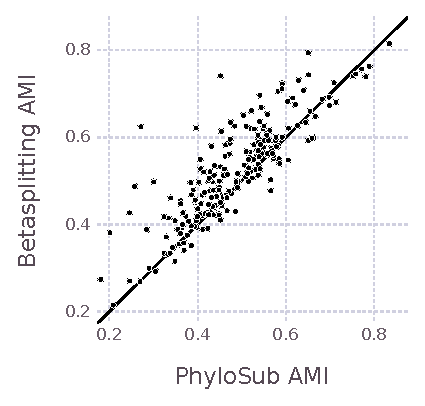
\includegraphics[width=0.9\columnwidth]{../figures/phylosub_betasplit_ami_scatter.eps}
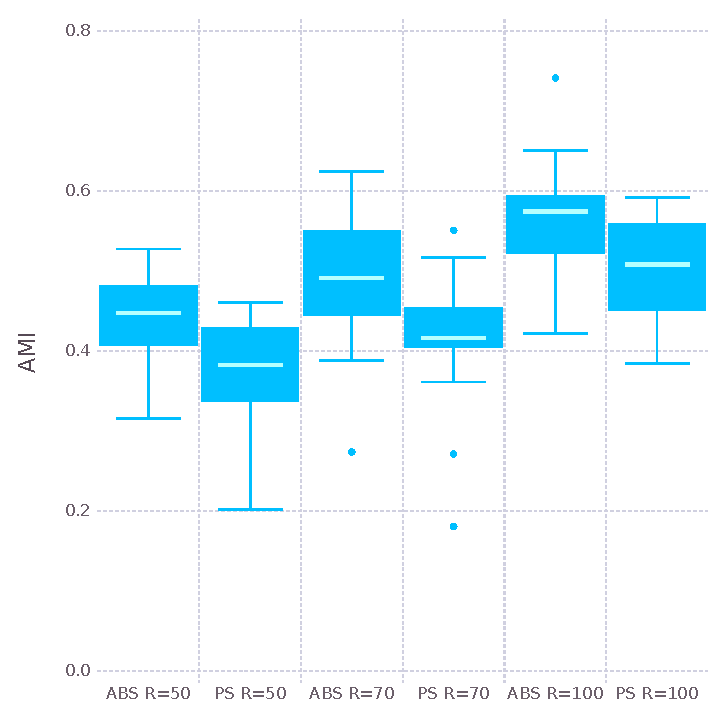
\includegraphics[width=0.9\columnwidth]{../figures/ami_boxplot_N_R.eps}
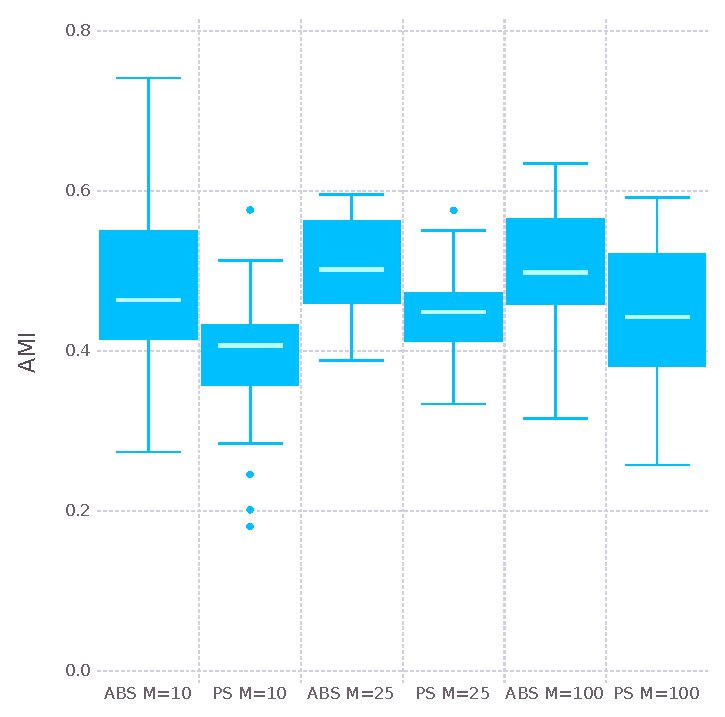
\includegraphics[width=0.9\columnwidth]{../figures/ami_boxplot_N_M.eps}
\caption{\textbf{(left)} Scatter plot showing the Adjusted Mutual Information for PhyloSub versus Aldous' Beta-Splitting.  \textbf{(center, right)} Effect of varying read depth and mutation number for the $K=5$ case.  ``ABS'' refers to Aldous' beta-splitting, ``PS'' refers to PhyloSub.}
\label{fig:scatter}
\end{figure}


We evaluated the two models by comparing the (flat) clusterings on the mutations to the ground truth clusterings, as in \cite{Jiao2014}.  However, \cite{Jiao2014} evaluates performance using area under the precision recall curve (AUPR) for the resulting co-clustering matrix.  We found that the AUPR measure of clustering quality overly penalizes clusterings with smaller numbers of clusters.   This preference for either small or large number of clusters is a common problem for cluster evaluation scores that don't account for the score that might have occurred due to chance \cite{Vinh2010}.  Thus, we depart from \cite{Jiao2014} and compare the two models using Adjusted Mutual Information (AMI) \cite{Vinh2009} on the flat clustering induced by the sampled hierarchies.  AMI is adjusted so that it does not generally prefer simple or complex models.

For a pair of partitions $C^{(1)}$ and $C^{(2)}$, define the distributions $p^{(k)} = C^{(k)}/|C^{(k)}|$.  Then the AMI is defined as
\begin{equation}
AMI(C^{(1)}, C^{(2)}) = \frac{I(p^{(1)}, p^{(2)}) - \mathbb{E}_q\left[I(p^{(1)}, p^{(2)})\right]  }{\max(H(p^{(1)}), H(p^{(2)})) - \mathbb{E}_q\left[I(p^{(1)}, p^{(2)})\right]}
\end{equation} 
where $H$ is entropy, $I$ is mutual information, and $q$ is a generalized hypergeometric distribution \cite{Vinh2009}.
%A partition $C = \{C_1, \ldots, C_k\}$ of a set $S$ can be viewed as a sample from a process in which the points in $S$ are assigned to the integers.  We can thus take the empirical distribution of the sample $C$ as $p_i := \frac{|C_i|}{|S|}$.  Likewise, given two partitions $C^{(1)}$ and $C^{(2)}$ on $S$, we can compute an empirical joint distribution by $p^{(1)(2)}_{i,j} = \frac{|C^{(1)}_i \cap C^{(2)}_j| }{|S|}$.  We can then compute the mutual information (MI): $I(C^{(1)}, C^{(2)}) = \mathbb{E}_{p} \log \frac{p^{(1)(2)}}{p^{(1)} p^{(2)}}$ in order to evaluate clusterings.  However, MI also prefers complex models to simple ones \cite{}.  Adjusted Mutual Information corrects this tendency by taking into account the amount of agreement that may occur between two clusterings due to chance under an assumed model of randomness:

To compare the two methods, we estimate the expected AMI:
\begin{equation}
\mathbb{E}\left[AMI(C, C^*)\right] \approx \frac{1}{W} \sum_{k=1}^K w_k AMI(C^{(k)}, C^*)
\end{equation}
where $C^{(k)}$ is the clustering associated with the $k$th MCMC sample, $C^*$ is the ground truth clustering, and $W=\sum_k w_k$.  $w_k = Z_{n_k}/L_{n_k}$, where $n_k$ is the WL block to which $k$ belongs, $Z_n$ is the WL partition function estimate associated with block $n$, and $L_n$ is the number of samples in block $n$.  In the case of PhyloSub, $w_k=1$.
 
As seen in Figure \ref{fig:scatter}, our model generally outperforms PhyloSub on AMI.  The difference in performance of the two algorithms did not have a strong dependence on read depth or mutation number.  However, PhyloSub's performance declines in the $K=5$ case.  Interestingly, this effect does not quickly diminish with the introduction of more data; see Figure \ref{fig:scatter}.  This suggests that either the PhyloSub model begins to fit poorly as data complexity increases, or that its sampler fails to mix in more complex settings.

%\subsection{Relationship between Time, Mutation Number, and Population Size}
%The generative description in Section \ref{sec:likelihood} implies that there is a relationship between mutation number and population size that we expect to see in real data.  Older subpopulations diverged from the reference population earlier, and are thus more likely to be large.  However, we expect to see a smaller number of mutations associated with older populations: as the lineage that gave rise to an older population had less time to acquire passenger mutations before the new subpopulation began to grow.  Thus, we expect an inverse relationship between mutation number and population size.
%
%The Beta-Splitting model is capable of modelling these subtle interactions through the relationship of the time variables $t$ and the population split proportions $\upsilon$.  These two variables are tied through $\nu$.  The length of the branch giving rise to subpopulation $i$ is $t_{\tau(i)}-t_i \propto 1-\nut_i \nu_i$, and $E[\upsilon_{i,s}] = \frac{\alpha \nu_i +1}{2+\alpha}$, so we do indeed find an inverse relationship between $t_i$ and $\upsilon_{i,s}$, and $\alpha$ controls the strength of this relationship.  When $\alpha=0$, $t$ and $\upsilon$ are independent.  


\section{Conclusion}
\label{sec:conclusions}
We have presented a model for subclonal reconstruction utilizing Aldous' beta-splitting as a prior on tree structures.  Marginalizing out the splitting locations that do not separate a finite set of points provides a compact representation for beta-splitting draws; furthermore, consistent time variables can be introduced to produce a projective prior over trees with times.  Additionally, we have leveraged the recursive structure of beta-splitting to develop an efficient MCMC sampler.  Applied to subclonal reconstruction, beta-splitting improves over the state of the art model.


\section*{Acknowledgements}

\section*{Funding}

This work has been supported by the... Text Text  Text Text.\vspace*{-12pt}

%\bibliographystyle{natbib}
%\bibliographystyle{achemnat}
%\bibliographystyle{plainnat}
%\bibliographystyle{abbrv}
%\bibliographystyle{bioinformatics}
%
%\bibliographystyle{plain}
%
%\bibliography{Document}

\newpage
\bibliography{../bibtex/library}
\bibliographystyle{plain}
%\newpage
%\onecolumn
%\subfile{beta_splitting_supplementary}

\end{document}
